\clearpage
%\fancyfood[R]{\thepage}
%\renewcommand{\headrulewidth}{0.5pt}
\setlength{\parindent}{1cm}     % Set paragraph indentation globally

\chapter{General Project Context}
\chaptermark{General Project Context}
\pagestyle{fancy}
\fancyhf{}
\fancyhead[HL]{Chapter 1: General Project Context}
\cfoot{\thepage}

\section{Introduction}
This chapter introduces the general context of the graduation project and the environment in which it was carried out. It begins with a presentation of the host company, Be Wireless Solutions (BWS), including its organization, areas of activity, and principal IoT solutions. The chapter then presents the project specifications by defining the identified problem, the concept of the IO-Box platform, the adopted development methodology, and the project's objectives and expected impact. This overview provides the necessary background for understanding the technical developments presented in the following chapters.

\section{Academic Institution}
The Higher Institute of Computer Science and Mathematics of the University of Monastir (ISIMM) is created by the decree n° 1623 of July 09, 2002, is a scientific, public higher education establishment, placed under the supervision of the Ministry of Higher Education and Scientific Research.

ISIMM offers educational programs in the field of Science and Technology that focus on the following disciplines: Computer Science, Mathematics and Electronics\cite{0}.

%__ Hosting company presentation 
\section{Host Company Presentation}

\subsection{Company Overview}
Be Wireless Solutions (BWS) is a Tunisian engineering company specialized in IoT systems, embedded electronics, and industrial monitoring platforms. The company develops end-to-end solutions combining embedded firmware, hardware design, and cloud-based supervision tools. Its engineering activities cover sensor integration, real-time data acquisition, and communication systems for industrial environments.\cite{1}.

The company designs and manufactures connected devices, communication gateways, smart sensors, and cloud-based platforms that enable real-time monitoring, control, and optimization of industrial processes and infrastructures. By combining hardware development, embedded software engineering, wireless communication technologies, and cloud services, BWS provides complete end-to-end IoT solutions adapted to various industrial sectors.

Since its creation, BWS has continuously expanded its activities and established collaborations both nationally and internationally. The company has developed expertise in industrial automation, energy management, smart agriculture, fleet management, environmental monitoring, and remote equipment supervision.

\begin{figure}[H]
    \centering
    
\includegraphics[width=0.4\textwidth]{Figures/bws_logo.png}
    \caption{Be Wireless Solutions (BWS) logo}
    \label{fig:bws_logo}
\end{figure}

\subsection{Organization Chart}
The organizational structure of BWS is composed of several departments that collaborate throughout the development lifecycle of industrial and IoT solutions. These departments include management, research and development, hardware design, embedded software development, cloud services, technical support, and business development.

\begin{figure}[H]
    \centering
    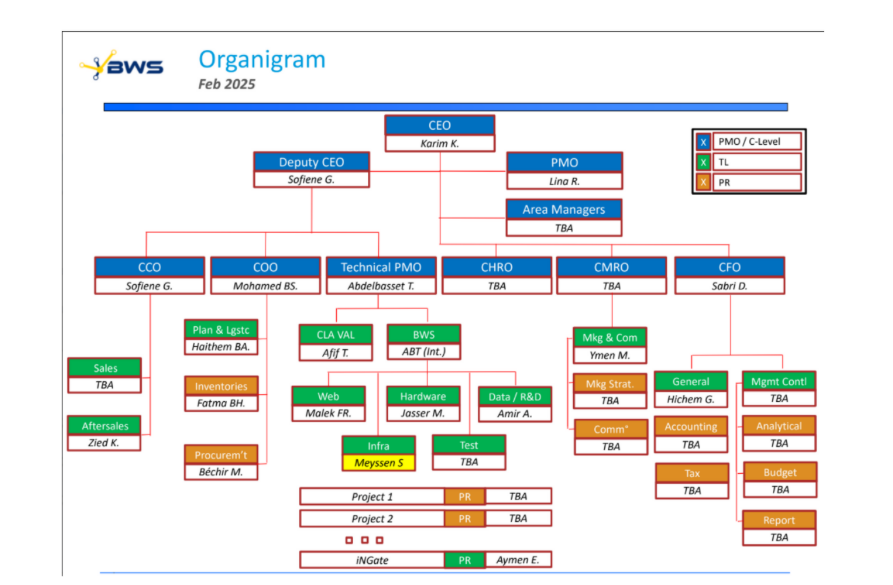
\includegraphics[width=0.75\textwidth]{Figures/organigram.png}
    \caption{Organization chart of Be Wireless Solutions}
    \label{fig:organization_chart}
\end{figure}

\subsection{Main Activities and Services}

BWS develops a wide range of industrial IoT solutions designed to improve operational efficiency, resource management, and process supervision.

\subsubsection{Energy Monitoring and Management}

BWS provides intelligent energy monitoring systems capable of collecting, analyzing, and visualizing electricity consumption data in real time. These solutions help organizations identify energy-intensive equipment, optimize consumption, reduce operational costs, and improve environmental performance.

\begin{figure}[H]
    \centering
    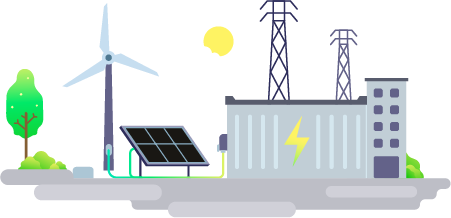
\includegraphics[width=0.7\textwidth]{Figures/electricity.png}
    \caption{Electricity consumption monitoring solution}
\end{figure}

\subsubsection{Water Monitoring Solutions}

The company offers smart water management solutions that enable remote meter reading, leak detection, abnormal consumption monitoring, and resource optimization.

\begin{figure}[H]
    \centering
    
\includegraphics[width=0.7\textwidth]{Figures/water.png}
    \caption{Water consumption monitoring solution}
\end{figure}

\subsubsection{Fleet and Fuel Management}

BWS develops fleet management systems that provide real-time vehicle tracking, fuel consumption analysis, route optimization, and driver behavior monitoring.

\begin{figure}[H]
    \centering
    
\includegraphics[width=0.7\textwidth]{Figures/fleet.png}
    \caption{Fleet and fuel management solution}
\end{figure}

\subsubsection{Remote Monitoring and Equipment Control}

The company provides remote supervision solutions that allow operators to monitor industrial equipment, detect anomalies, generate alerts, and perform remote control operations through dedicated software platforms.

\begin{figure}[H]
    \centering
    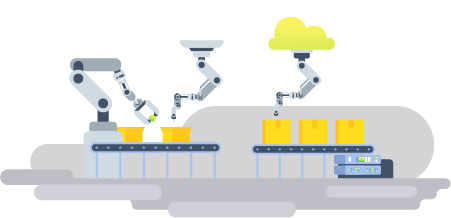
\includegraphics[width=0.7\textwidth]{Figures/equipment.png}
    \caption{Remote equipment monitoring and control}
\end{figure}

\subsubsection{Cold Chain Monitoring}

BWS also offers cold-chain monitoring systems intended for warehouses, refrigerated transportation, and pharmaceutical storage facilities. These solutions ensure compliance with temperature requirements and provide instant alerts when abnormal conditions occur.

\begin{figure}[H]
    \centering
    
\includegraphics[width=0.7\textwidth]{Figures/coldchain.png}
    \caption{Cold-chain monitoring solution}
\end{figure}

%__ Project specification
\section{Project Specification}

\subsection{Problem Statement}

Industrial IoT systems generally integrate a large number of sensors, actuators, and communication interfaces. In many cases, each new application requires dedicated firmware modifications, peripheral configuration, and hardware adaptations. This approach increases development time, reduces software reusability, and complicates system maintenance.

Moreover, industrial environments often involve heterogeneous communication protocols and interface standards. Managing these technologies through application-specific implementations creates additional complexity and limits system scalability.

To address these limitations, Be Wireless Solutions initiated the development of the IO-Box platform. The objective is to provide a configurable and reusable industrial acquisition and control system capable of simplifying peripheral integration while maintaining flexibility, portability, and maintainability.

\subsection{Presentation of the IO-Box Platform}

The IO-Box is a configurable industrial acquisition and control platform developed to facilitate the integration of sensors, actuators, and communication interfaces within industrial systems.

The platform is built around a modular embedded architecture that separates hardware-dependent components from application-level services. This approach relies on dedicated drivers, a Board Support Package (BSP), and Hardware Abstraction Layer (HAL) mechanisms to ensure portability and maintainability.

The IO-Box supports multiple categories of industrial peripherals, including analog inputs, digital inputs, digital outputs, communication interfaces, and measurement devices. Through a configurable software architecture, the platform can be adapted to different industrial use cases without significant firmware modifications.

By providing a unified interface between hardware resources and application services, the IO-Box reduces integration complexity and accelerates deployment in industrial environments.

\subsection{Project Objectives}

The main objective of this project is the design and development of the IO-Box platform capable of acquiring, processing, regulating, and transmitting industrial data in real time.

More specifically, the project aims to:

\begin{itemize}
    \item Design and implement a modular industrial acquisition and control platform.
    \item Provide a unified software abstraction layer for heterogeneous peripherals.
    \item Support configurable analog and digital input/output functionalities.
    \item Facilitate communication with external systems through industrial and IoT communication interfaces.
    \item Develop a modular software architecture based on abstraction layers and reusable software components.
    \item Ensure platform scalability for future industrial applications and system extensions.
\end{itemize}

\subsection{Development Methodology}

The development of the IO-Box platform follows the V-Model (Verification and Validation Model), a structured development methodology widely used in embedded and industrial systems.

The V-Model establishes a direct relationship between each development phase and its corresponding verification activity. This approach ensures complete traceability between system requirements, design decisions, implementation activities, and validation tests.

The descending branch of the model includes requirement analysis, system design, and software design activities. The implementation phase constitutes the central stage of the development cycle.

The ascending branch focuses on verification and validation through unit testing, integration testing, system testing, and final acceptance testing.

The adoption of the V-Model contributes to improving software quality, reducing development risks, and facilitating project management throughout the entire lifecycle.

\begin{figure}[H]
    \centering
    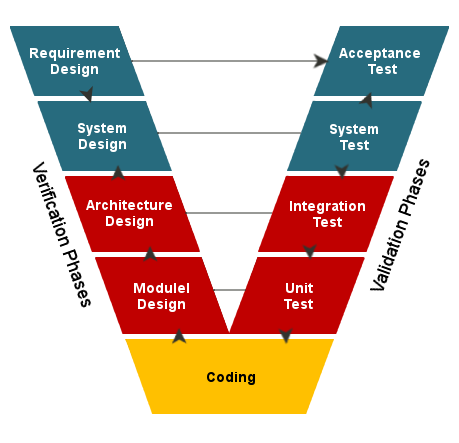
\includegraphics[width=0.75\textwidth]{Figures/v-model.png}
    \caption{V-Model development lifecycle}
    \label{fig:vmodel}
\end{figure}

\subsection{Expected Contributions}

The developed IO-Box platform is expected to significantly simplify the integration of industrial sensors and actuators while reducing deployment and maintenance efforts.

By providing a unified hardware and software architecture, the platform improves interoperability between devices and facilitates future system extensions. Furthermore, its modular design promotes software reuse and accelerates the development of new industrial applications.

The developed platform contributes to reducing development effort and deployment time by providing a standardized and reusable embedded architecture capable of supporting a wide range of industrial applications.

\section{Conclusion}

This chapter introduced the general framework of the project. The academic institution and the host company were first presented, followed by an overview of the company's activities and technological solutions. The project specifications, problem statement, objectives, and development methodology were then detailed.

The next chapter focuses on the requirements analysis and system study, providing a detailed description of the functional and technical requirements that guided the design and implementation of the IO-Box platform.